\documentclass[a4paper]{article}
\usepackage[warn]{mathtext}
\usepackage[utf8]{inputenc}
\usepackage[T2A]{fontenc}
\usepackage[english,russian]{babel}
\usepackage{multicol}
\usepackage{fancyhdr}
\usepackage{graphicx}
\usepackage{microtype}
\usepackage{wrapfig}
\usepackage{amsmath}
\usepackage{floatflt}
\usepackage{geometry} \geometry{verbose,a4paper,tmargin=2cm,bmargin=2cm,lmargin=1.5cm,rmargin=1.5cm}
\usepackage{float}
\usepackage{amssymb}
\usepackage{caption}
\usepackage{epsfig}
\usepackage{newunicodechar}

\begin{document}

\graphicspath{ {pictures/} }

\begin{titlepage}
	\centering
	\vspace{5cm}
    {\scshape\LARGE Московский физико-технический институт\par}
	\vspace{5cm}
	{\scshape\Large Лабораторная работа по радиотехнике \par}
	\vspace{1cm}
    {\huge\bfseries  №28 Усилитель на биполярных транзисторах \par}
	\vspace{1cm}
	\vfill
    \begin{flushright}
        {\large выполнил студент Б04-852 группы ФЭФМ}\par
        \vspace{0.3cm}
        {\LARGE Яромир Водзяновский}
    \end{flushright}
	\vfill
Долгопрудный, 2021
% Bottom of the page
\end{titlepage}

\pagestyle{fancy} 
\fancyhead[L]{Радиотехника   $\sim  \hat(\, ^{\circ}  \omega  ^{\circ} \, \hat) \sim$}
% \fancyhead[L]{Закон Кюри-Вейса    $( *{^\circ}< >^{\circ}*)$}
\fancyhead[R]{Лабораторная работа}
\fancyhead[C]{}
\fancyfoot[C]{ \noindent\rule{\textwidth}{0.4pt} \thepage }

\newcommand{\ap}{\approx}
\newcommand{\cb}[1]{\begin{center}\fbox{#1} \end{center}}
\newcommand{\cc}[1]{\begin{center} #1 \end{center}}

\newpage



\textbf{Задание:} На заданных значениях: 
\begin{center}
    \fbox{$R_k = 3.9\; кОм,\;I_k = 2.5\; мА, \; C_б = 200\; нФ$, $U_п = 10В$ }
\end{center}

рассчитаем, соберем и исследуем указанные схемы, измеряя совокупность параметров:

\begin{equation}
    U_{вых. макс}, \; K_u, \; K_e,\; R_{вх}, \; f_н, \; f_в
\end{equation}



\

\begin{center}
    \scshape\large\textbf{Нестабилизированный усилитель}
\end{center}

\begin{enumerate}

    \item  Соберем схему (рис. \ref{sch1}), установим $R_б = \hat{R}_б \ap 200 \cdot R_k$, чтобы ток $I_k$ равнялся заданному $\hat{I}_k$. Измерим $U_{кэ}$ и $U_{бэ}$. Найдем $h_{21э}$.  \par 
    
    \begin{figure}[H]
        \begin{center}
            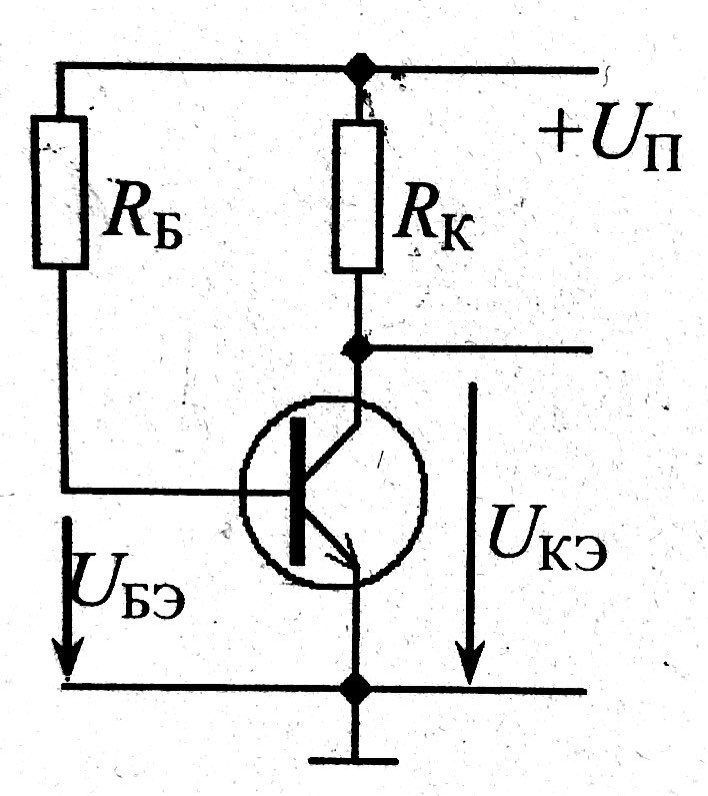
\includegraphics[scale = 0.1]{1_1.jpg}
            \caption{Схема 1}
            \label{sch1}
        \end{center}
    \end{figure}

        \begin{enumerate}
            \item Измеренные значения напряжений:
                \begin{center}
                    \fbox{$U_{кэ} \ap 6.13\;В \;\;\;\;\;\; U_{бэ} \approx 0.64\; В$}
                \end{center}
            
            \item Определим $I_k$ и $I_б$ измерив падение напряжение и зная сопротивление:
            $$I_k \ap 1.5\; мА  \;\;\;\;\;\; I_б \ap 11.4 \; мкА$$
                
            \item Посчитаем $h_{21э}$ по следуюзщей формуле:
                \begin{center}
                    \fbox{$h_{21э} = I_k/I_б \ap 131$}
                \end{center}

            \item Определим $R_б$ и сравним с даным значением:
            $$R_б = h_{21э} (U_п - U_{бэ})/\hat{I}_k \ap 492\; кОм$$

        \end{enumerate}


    \item Соберем схему (рис. \ref{sch2}). Для нестабилизированного усилителя с $R_и \ap R_k$ определим параметры (1) при $R_б = \hat{R}_б$ и при $R_б = 2 \cdot \hat{R}_б$ \par 
    
    \begin{figure}[H]
        \begin{center}
            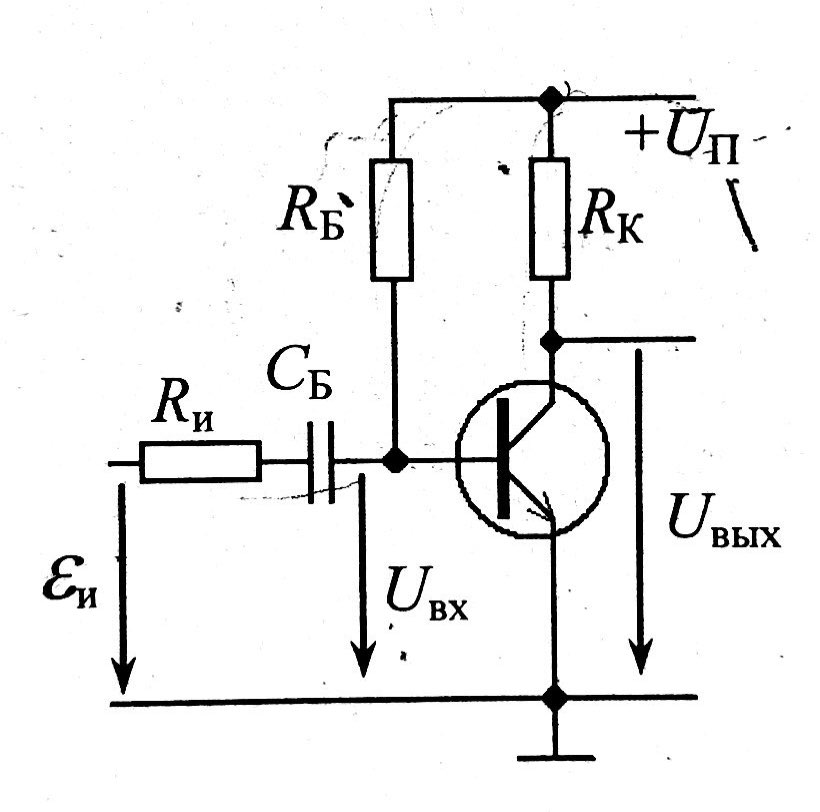
\includegraphics[scale = 0.15]{2_1.jpg}
            \caption{Схема 2}
            \label{sch2}
        \end{center}
    \end{figure}

        \begin{itemize}
            \item \textbf{$R_б = \hat{R}_б = 492\; кОм$}
                \begin{enumerate}
                    \item Измерим $U_{вых. макс}, \; U_{вх}$ :
                    \cb{$U_{вых. макс} = 13.9\; В$}
                    \cc{$U_{вх} = 1.7 \; В$}

                    \item Определим $K_u, \; K_e$:
                    \cb{$K_u = U_{вых}/U_{вх} = 8.3 \;\;\;\;\; K_e = U_{вых}/E_u  = 7$}

                    \item Определим $R_{вх}$:
                    \cb{$R_{вх} = \frac{U_{вх} R_u}{\Delta U_{R_u}} \ap 15\; кОм$}

                    \item Верхняя и нижняя пороговые частоты определяются исходя из падения амплитуды сигнала в $\ap 0.7$ раз:
                    \cb{$f_н \ap 330\; Гц \;\;\;\;\;\; f_в \ap 1\; МГц$}
                \end{enumerate}
            
            \item \textbf{$R_б = 2 \cdot \hat{R}_б = 820\; кОм$}
                \begin{enumerate}
                    \item Измерим $U_{вых. макс}, \; U_{вх}$ :
                    \cb{$U_{вых. макс} = 13.3\; В$}
                    \cc{$U_{вх} = 1.8 \; В$}

                    \item Определим $K_u, \; K_e$:
                    \cb{$K_u = U_{вых}/U_{вх} = 7.4 \;\;\;\;\; K_e = U_{вых}/E_u  = 6.7$}

                    \item Определим $R_{вх}$:
                    \cb{$R_{вх} = \frac{U_{вх} R_u}{\Delta U_{R_u}} \ap 28\; кОм$}

                    \item Верхняя и нижняя пороговые частоты определяются исходя из падения амплитуды сигнала в $\ap 0.7$ раз:
                    \cb{$f_н \ap 8\; Гц \;\;\;\;\;\; f_в \ap 1.4\; МГц$}
                \end{enumerate}

        \end{itemize}

    
    \item Соберем схему (рис. \ref{sch3}). Определим параметры (1) нестабилизированного усилителя с внешней нагрузкой $R_н \ap R_k$ при $R_б = \hat{R}_б$ и $C_э \geq 100\; мкФ$.
    
    \begin{figure}[H]
        \begin{center}
            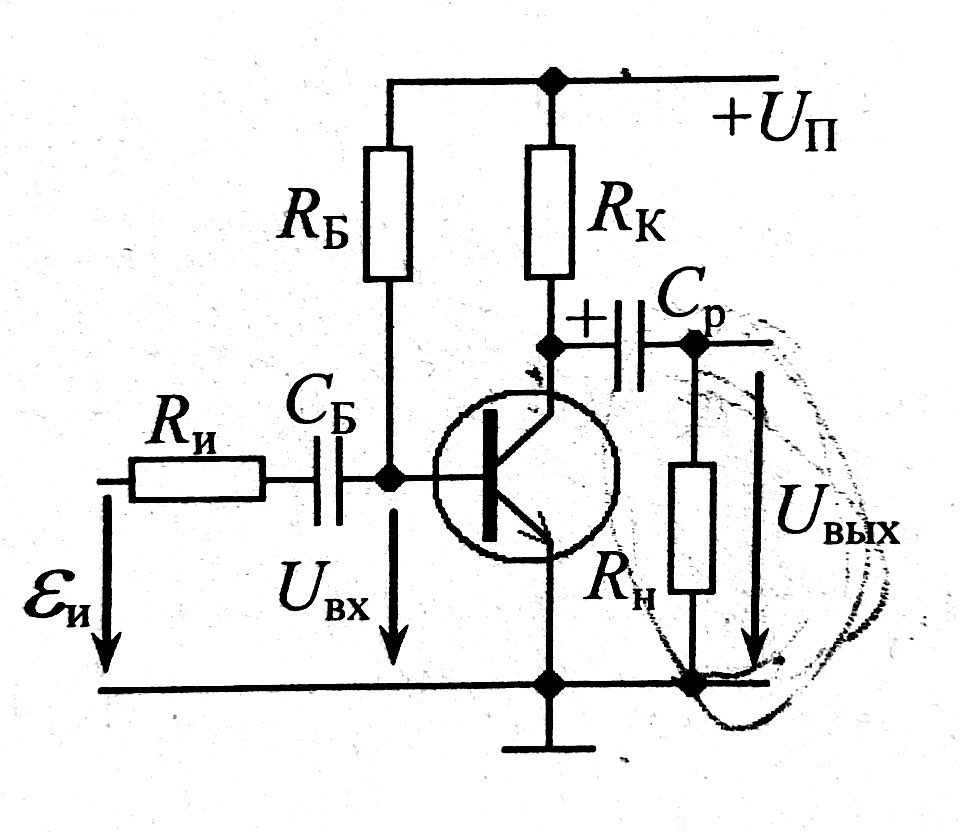
\includegraphics[scale = 0.15]{3_1.jpg}
            \caption{Схема 3}
            \label{sch3}
        \end{center}
    \end{figure}

        \begin{enumerate}
            \item Измерим $U_{вых. макс}, \; U_{вх}$ :
            \cb{$U_{вых. макс} = 0.69\; В$}
            \cc{$U_{вх} = 0.11 \; В$}

            \item Определим $K_u, \; K_e$:
            \cb{$K_u = U_{вых}/U_{вх} = 6.27 \;\;\;\;\; K_e = U_{вых}/E_u  = 4.92$}

            \item Определим $R_{вх}$:
            \cb{$R_{вх} = \frac{U_{вх} R_u}{\Delta U_{R_u}} \ap 14\; кОм$}

            \item Верхняя и нижняя пороговые частоты определяются исходя из падения амплитуды сигнала в $\ap 0.7$ раз:
            \cb{$f_н \ap 42\; Гц \;\;\;\;\;\; f_в \ap 600\; кГц$}
        \end{enumerate}

\

\

\begin{center}
    \scshape\large\textbf{Cтабилизированный усилитель}
\end{center}

\

    \item Соберем схему (рис. \ref{sch4}). Выберем $R_э = 910\; Ом, \;\;\;R_2 = 6,8\; кОм$. Бужем подбирать $R_1$ из условия получения заданного тока коллектора $\hat{I}_k$. Измерить $U_б, \; U_э, \; U_k$ относительно земли.

    \begin{figure}[H]
        \begin{center}
            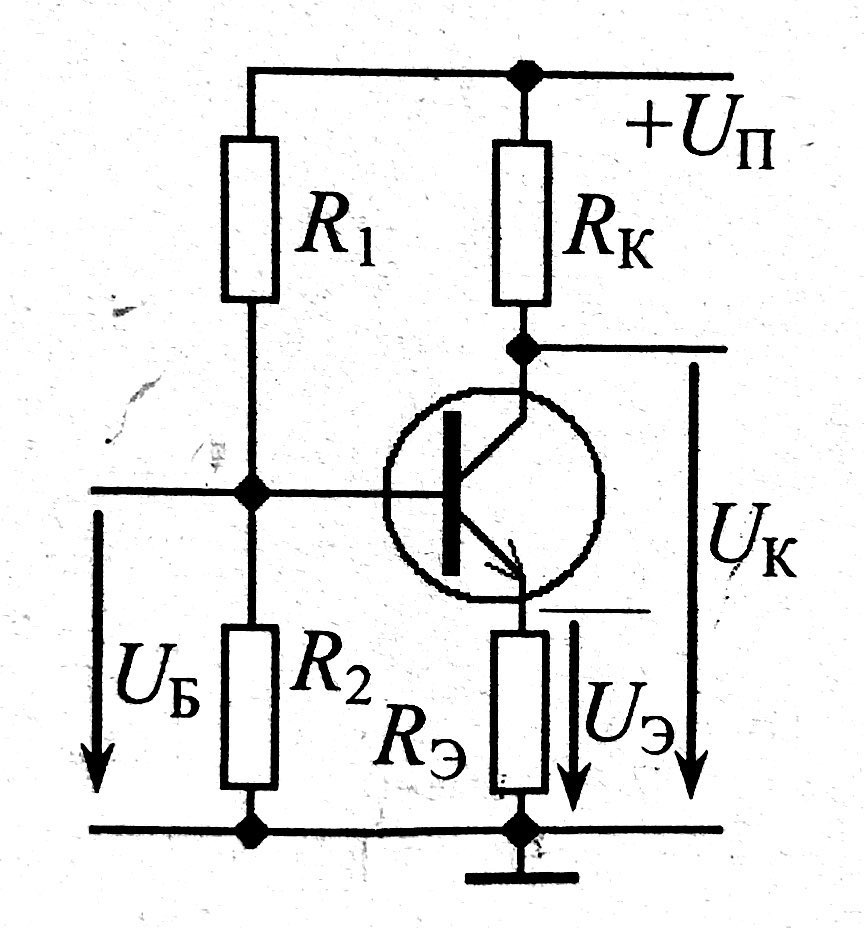
\includegraphics[scale = 0.15]{4_1.jpg}
            \caption{Схема 4}
            \label{sch4}
        \end{center}
    \end{figure}

        \begin{enumerate}
            \item Условие получения заданного тока коллектора: 
            \cc{$I_k \approx (U_б - U_{бэ})/R_э$}
            В нашем случае будем подбирать $R_1$ так, чтобы выполнилось условие:
            \cc{$(U_б - U_{бэ}) \approx 1.365\; В$}

            \item Получим нужное сопротивление:
            \cb{$R_1 = 3.6\; кОм$}

            \item Измерим напряжения:
            \cb{$U_б = 1.97\;В, \;\;\; U_э = 1.32\;В, \;\;\; U_k = 1.4\; В$}
        \end{enumerate}

\

\cc{\scshape\large Далее будет другое напряжение $U_п = 5 \;В$}

\

    \item Соберем схему (рис. \ref{sch5}). Для данной схемы $C_э \geq 100\; мкФ$ определим параметры (1) при $R_и \ap R_k$.

    \begin{figure}[H]
        \begin{center}
            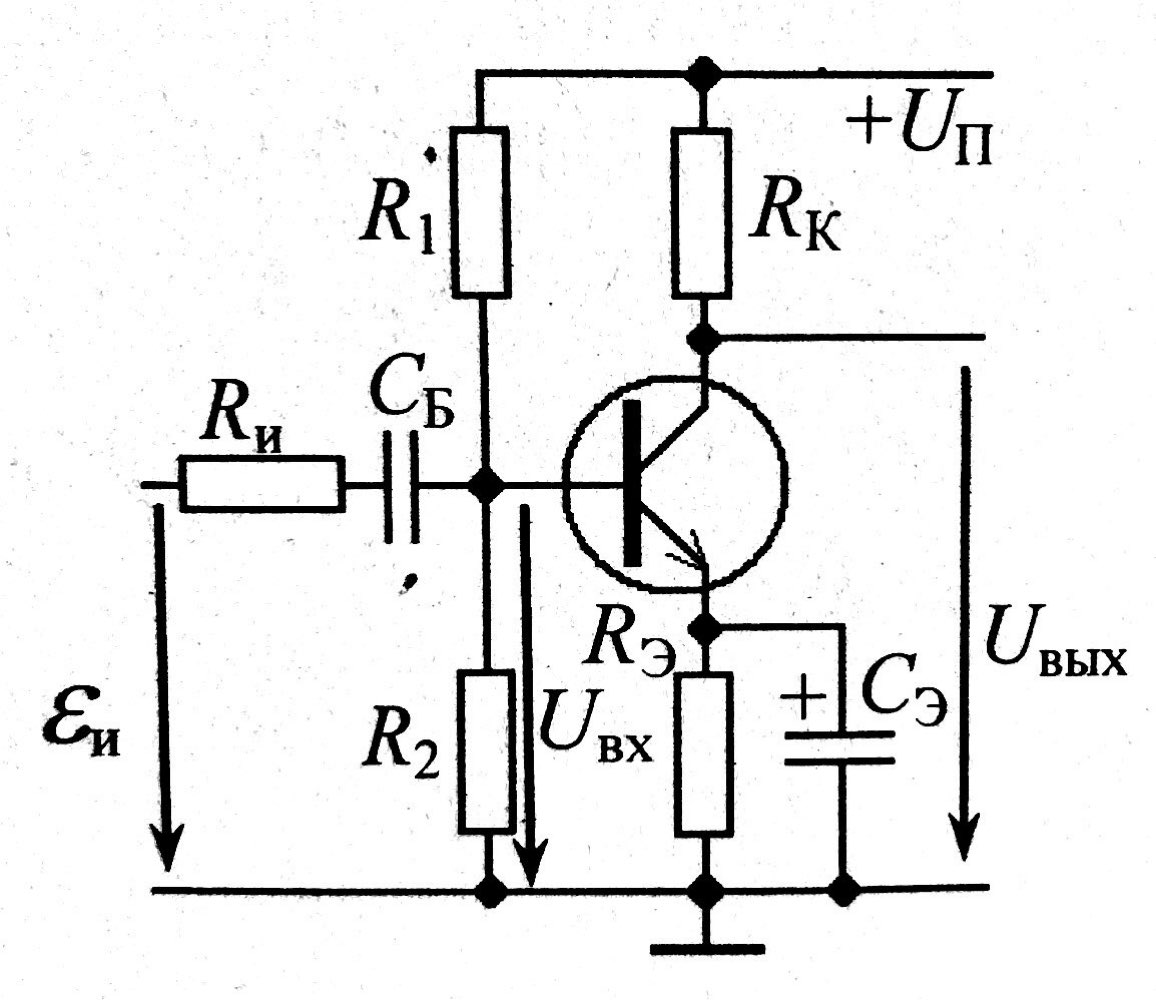
\includegraphics[scale = 0.15]{5_1.jpg}
            \caption{Схема 5}
            \label{sch5}
        \end{center}
    \end{figure}

        \begin{enumerate}
            \item Измерим $U_{вых. макс}, \; U_{вх}$ :
            \cb{$U_{вых. макс} = 0.173\; В$}
            \cc{$U_{вх} = 0.025 \; В$}
            \cc{$E_u \ap 0.314\; В$}

            \item Определим $K_u, \; K_e$:
            \cb{$K_u = U_{вых}/U_{вх} = 6.92 \;\;\;\;\; K_e = U_{вых}/E_u  = 0.5$}

            \item Определим $R_{вх}$:
            \cb{$R_{вх} = \frac{U_{вх} R_u}{\Delta U_{R_u}} \ap 337.4\; Ом$}

            \item Верхняя и нижняя пороговые частоты определяются исходя из падения амплитуды сигнала в $\ap 0.7$ раз:
            \cb{$f_н \ap 370\; Гц \;\;\;\;\;\; f_в \ap 590\; кГц$}
        \end{enumerate}


    \item Работаем с предыдущей схемой (рис. \ref{sch5}). Подадим на вход усилителя прямоугольные колебания с периодом $T$ и пронаблюдаем выходной сигнал при $T \approx 15 \cdot \frac{1}{2 \pi f_н}$ и при $T \approx 15 \cdot \frac{1}{2 \pi f_в}$.

        Как мы знаем сигнал затухает экспоненциально:

        \begin{equation}
            U \sim e^{-t/\tau}
        \end{equation}

        Тогда прологарифмировав отношения для двух точек:

        \begin{equation}
            \tau = \frac{|t_1 - t_2|}{\ln{\frac{U_2}{U_1}}}
            \label{tau}
        \end{equation}

        \begin{figure}[H]
            \begin{center}
            \begin{minipage}[h]{0.4\linewidth}
            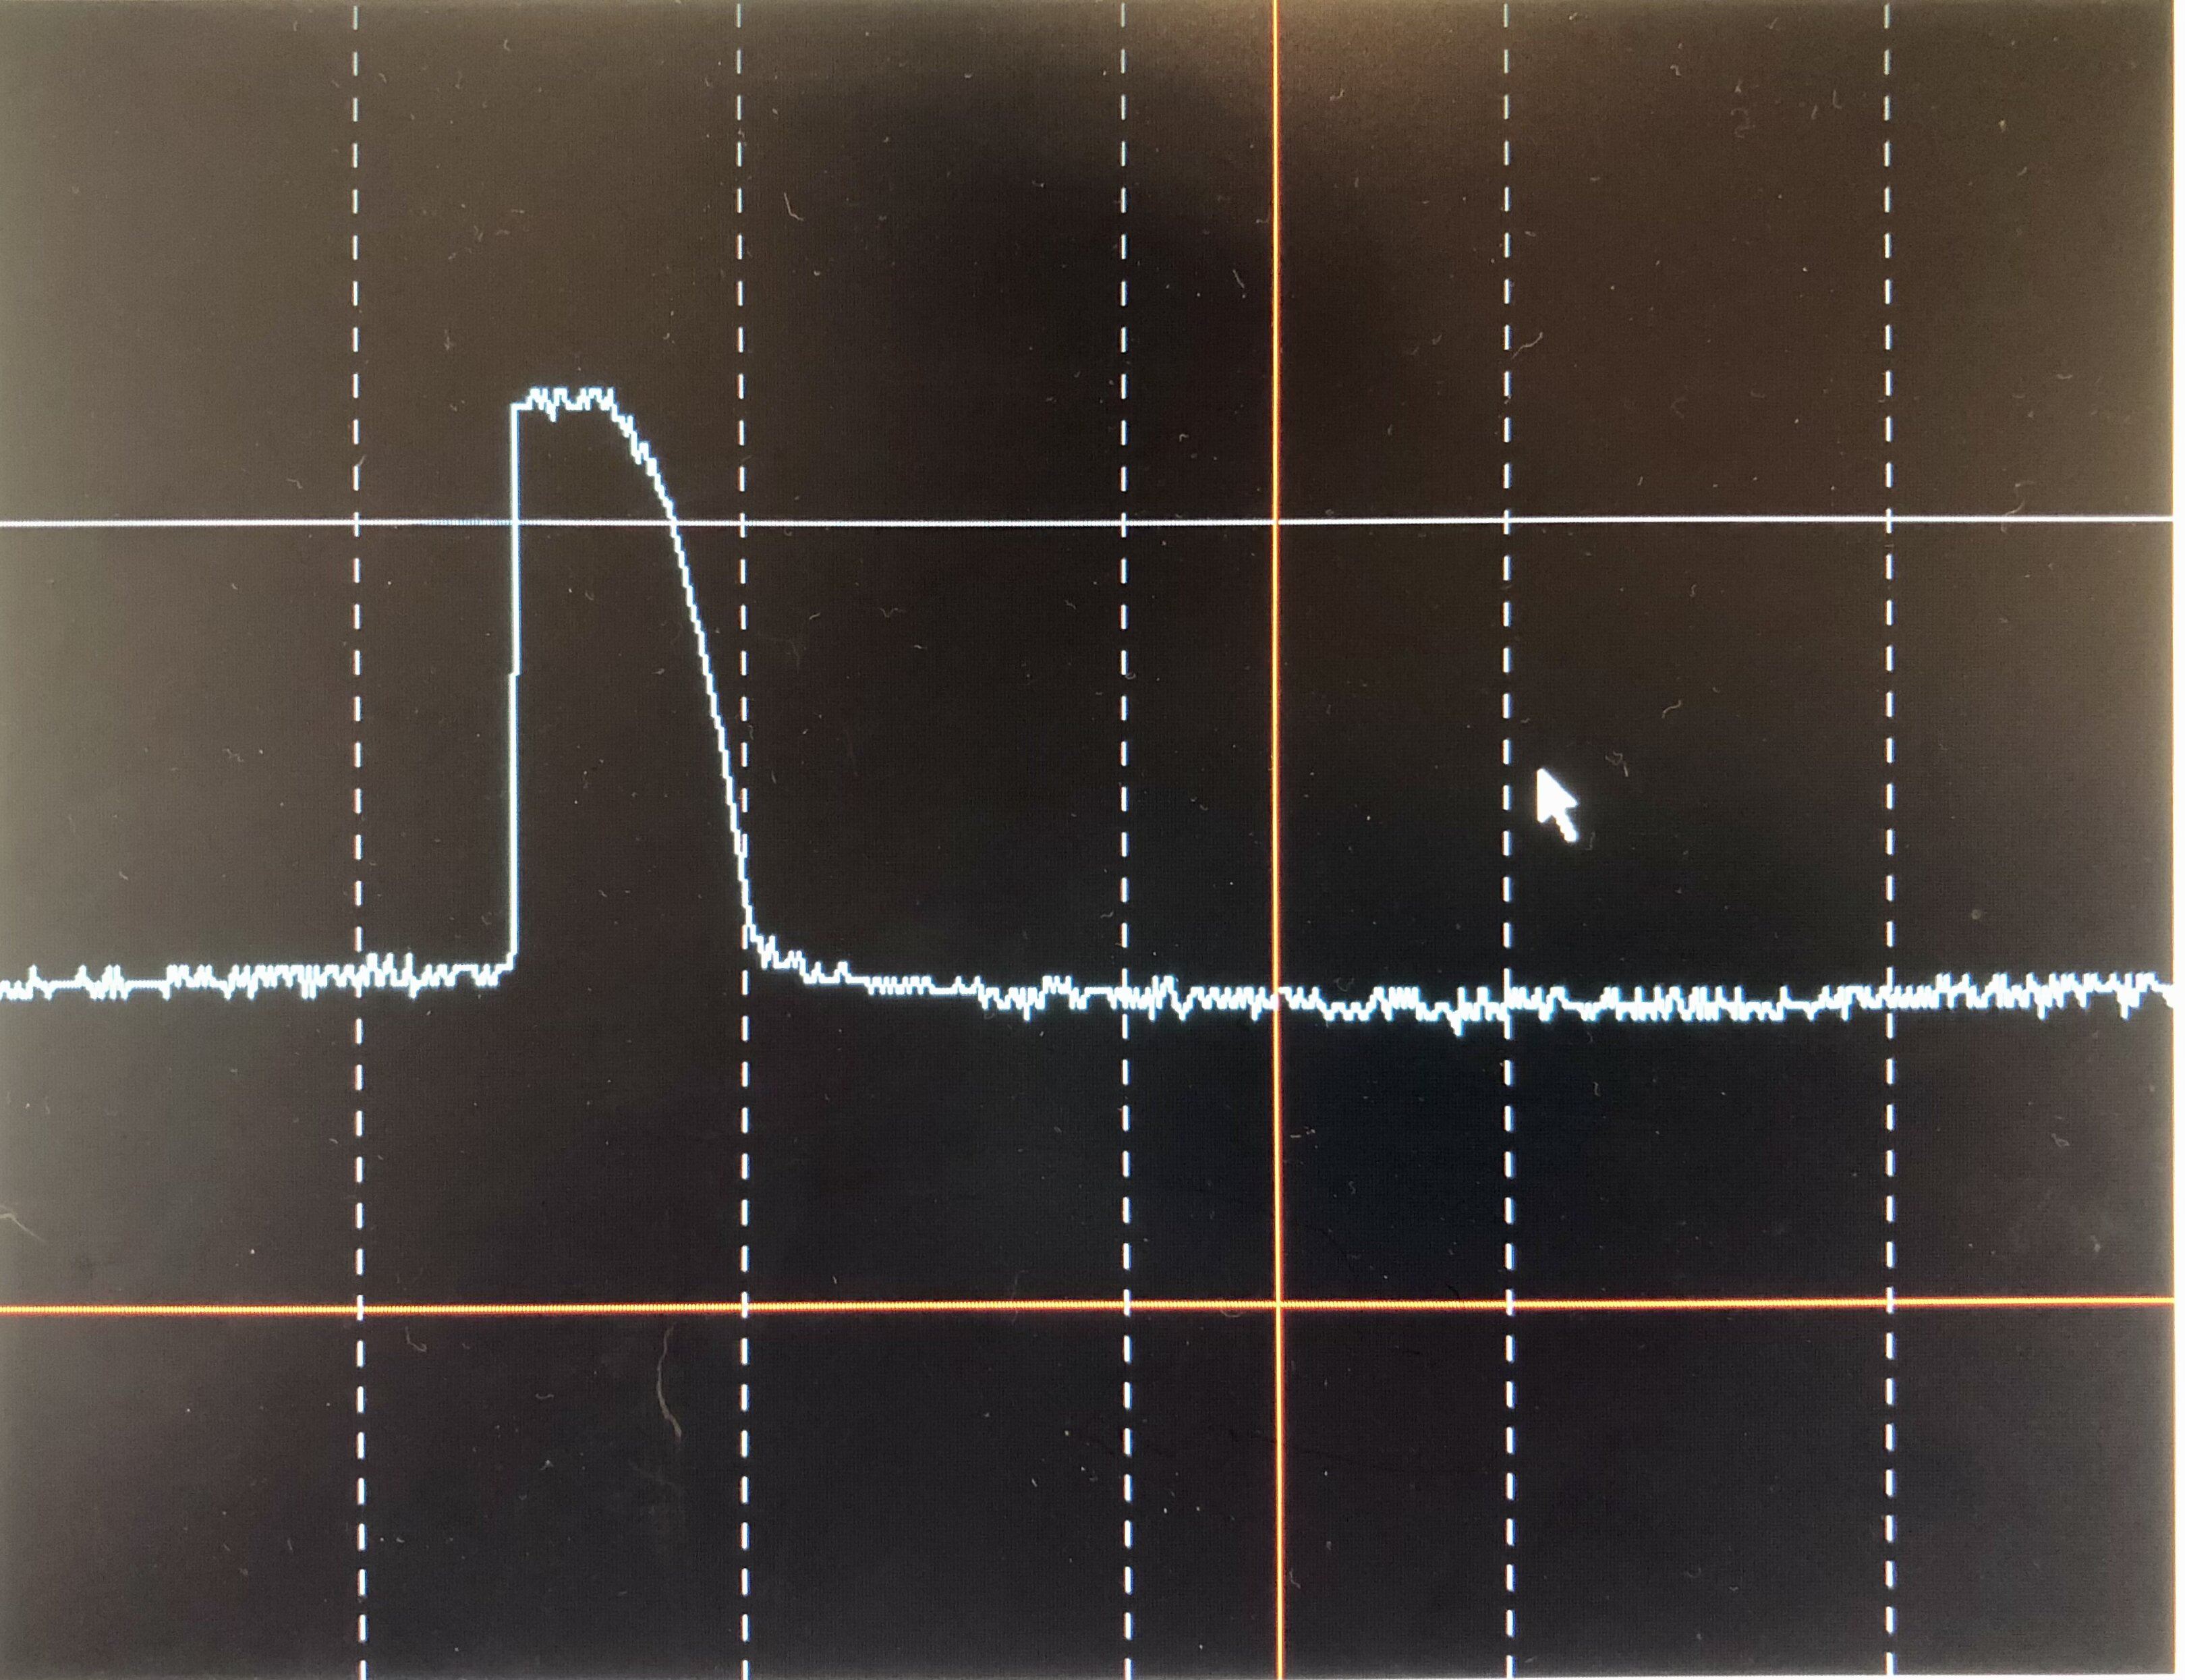
\includegraphics[width=1\linewidth]{f_n.jpg}
            \caption{Сигнал на осциллографе при нижней частоте} 
            \label{f_n}
            \end{minipage}
            \hfill 
            \begin{minipage}[h]{0.45\linewidth}
            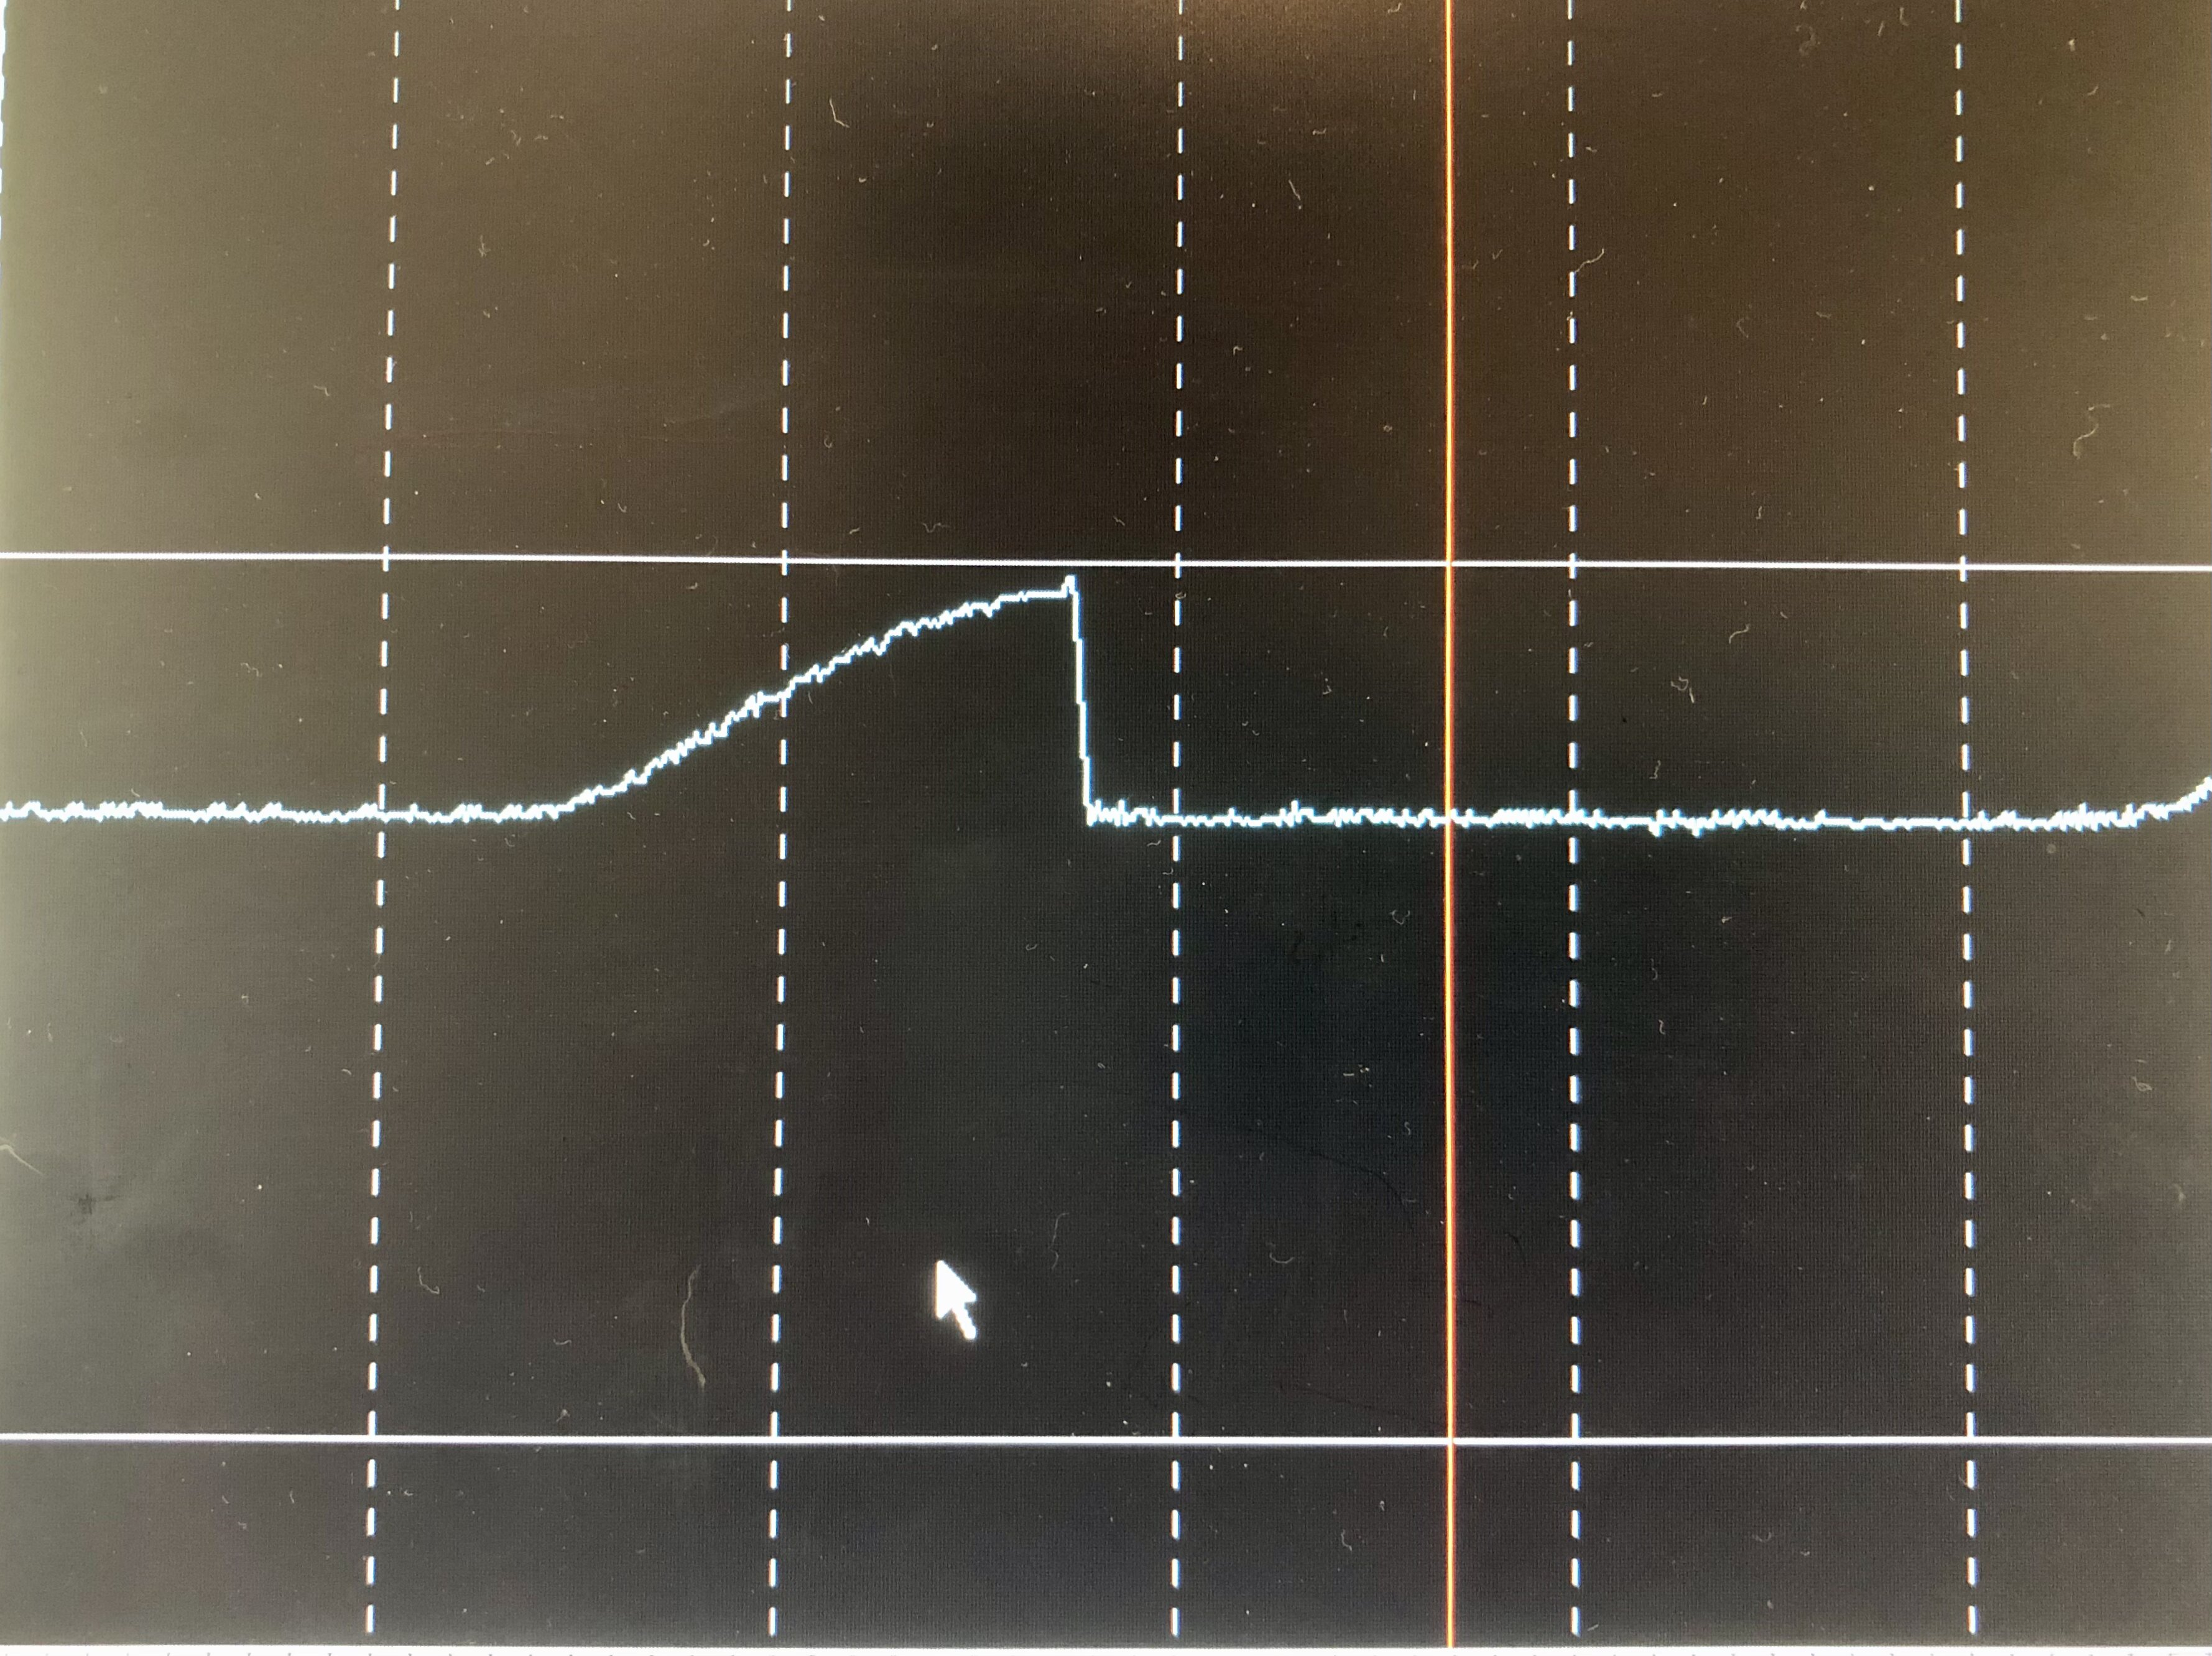
\includegraphics[width=1\linewidth]{f_v.jpg}
            \caption{Сигнал на осциллографе при высокой частоте}
            \label{f_v}
            \end{minipage}
            \end{center}
        \end{figure}

            \begin{itemize}
                \item $T \approx 15 \cdot \frac{1}{2 \pi f_н}$, $\nu_н \ap 153.8\; Гц$ \par 
                    По формуле (\ref{tau}) выберем 2 точки с графика на рис. \ref{f_n}:
                    \cb{$\tau_н \ap 0.42\; с$}
                
                \item $T \approx 15 \cdot \frac{1}{2 \pi f_в}$, $\nu_в \ap 250\; кГц$ \par
                    По формуле (\ref{tau}) выберем 2 точки с графика на рис. \ref{f_v}:
                    \cb{$\tau_в \ap 20.6 \cdot 10^{-3}\; с$}
                    
            \end{itemize}



    \item Соберем схему (рис. \ref{sch6}). Определим параметры (1) в стабилизированном усилителе с $C_э = 0$.

    \begin{figure}[H]
        \begin{center}
            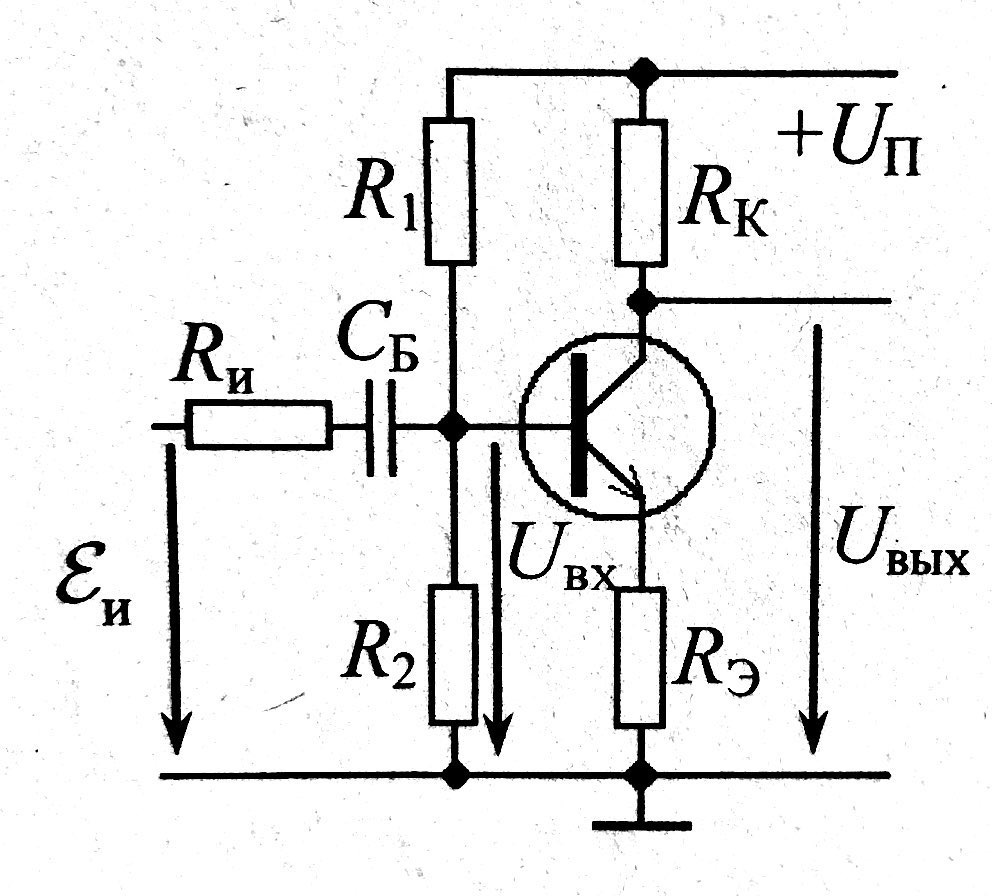
\includegraphics[scale = 0.15]{6_1.jpg}
            \caption{Схема 6}
            \label{sch6}
        \end{center}
    \end{figure}

        \begin{enumerate}
            \item Измерим $U_{вых. макс}, \; U_{вх}$ :
            \cb{$U_{вых. макс} = 45\; мВ$}
            \cc{$U_{вх} = 46 \; мВ$}
            \cc{$E_u \ap 320\; мВ$}

            \item Определим $K_u, \; K_e$:
            \cb{$K_u = U_{вых}/U_{вх} \ap 1 \;\;\;\;\; K_e = U_{вых}/E_u  \ap 0.14$}

            \item Определим $R_{вх}$:
            \cb{$R_{вх} = \frac{U_{вх} R_u}{\Delta U_{R_u}} \ap 654\; Ом$}

            \item Верхняя и нижняя пороговые частоты определяются исходя из падения амплитуды сигнала в $\ap 0.7$ раз:
            \cb{$f_н \ap 148\; Гц \;\;\;\;\;\; f_в \ap 5.8\; МГц$}
        \end{enumerate}


\end{enumerate}

\textbf{Выводы:}

\begin{enumerate}
    \item Собраны и изучены схемы нестабилизированного и стабилизированного усилителей.
    \item Определены коэффициенты транзистора на экспериментальных данных, значения попадают в реальные значения.
    \item Определены граничные частоты для транзистора.
    \item В ходе работы происходила замена рабочего месат, ввиду чего есть различия в снятых данных, также получились сильно отклоняющиеся от действительности значения для коэффициента усиления. 
\end{enumerate}


\end{document}